


\begin{center}

\chapter{ Contexte général du projet} 
	
\end{center}

Cette partie nous permet de présenterles circonstances de notre projet d’une manière générale, vous allez découvrir le sujet, les besoins et la planification du projet.\\ 


\section{Présentation du sujet}

L' E-Shopping est devenue un secteur très riche en innovation et en créativité c’est ce que nous a attirer vers ce domaine puisqu’il lie deux grands volés différents qui sont l’informatique et le shopping, ce mélange se présente dans notre projet qui est la mise en place d’une platfrome web qui facilite le shopping en recommandant aux utilisateurs des appareils convenables avec leurs besoins.\\

La platfrome TechGadgets cible le problème de passer plusieurs heures et même jours en cherchant dans l'internet un gadget qui satisfait nos besoins et résout également la nécessite d'avoir beaucoup de connaissances dans le domaine de technologie et matériel informatique. L'utilisateur aura le choix d'inscrire au bien choisir le "guest mode" pour accéder à notre service qui sera une recommandation des gadgets en se basant sur une description d'utilisateur. \\

L’application n’arrête pas ici, mais elle dépasse tout ça pour offrir l’option d'obtenir des recommandations plus personnalise pour les abonnes en utilisant l'histoire des transactions ainsi que la description.

\section{Besoins fonctionnels}

\underline {Coté Guest : }
\\
\begin{itemize}
  \item Description d'un Tech-Gadget
  \item Obtenir une liste des produits \\
\end{itemize}

\\

\underline {Coté abonné : }
\\
\begin{itemize} 

    \item Authentification
    \item Description d'un Tech-Gadget
    \item Obtenir une liste des produits
    \item Évaluer Les resultats \\
\end{itemize}
\\

\section{Besoins non fonctionnels}

Une fois traiter le coté fonctionnel , nous devons considérer aussi les besoins non fonctionnels , par exemple : \\

\begin{itemize}
    \item User experience
    \item Actualisation des informations
    \item Maximum de sécurité 
    \item Adaptation à l'utilisateur 
\end{itemize}


\begin{center}
\chapter{Analyse et conception}    
\end{center}

Ce chapitre présente l'analyse théorique de notre projet. \\
\section{Acteurs :}

Les acteurs  de notre application sont principalement comme suit : \\

\textbf{Le développeur} : Il gère les comptes des utilisateurs, il peut aussi ajouter des services à l'application( Ajouter la recherche du produit dans Jumia par exemple, améliorer le model NLP )

\textbf{L'utilisateur} : Chercher un produit sur Internet à l'aide d'un texte descriptif, en précisant les sites ciblés dans son recherche 

\section{Diagramme des cas d’utilisation ;}

Un diagramme de cas d'utilisation capture le comportement d'un système, d'un sous-système, d'une classe ou d'un composant tel qu'un utilisateur extérieur le voit. Il scinde la fonctionnalité du système en unités cohérentes, les cas d'utilisation, ayant un sens pour les acteurs. Les cas d'utilisation permettent d'exprimer le besoin des utilisateurs d'un système, ils sont donc une vision orientée utilisateur de ce besoin au contraire d'une vision informatique.

\begin{figure}[h]
    \centering
    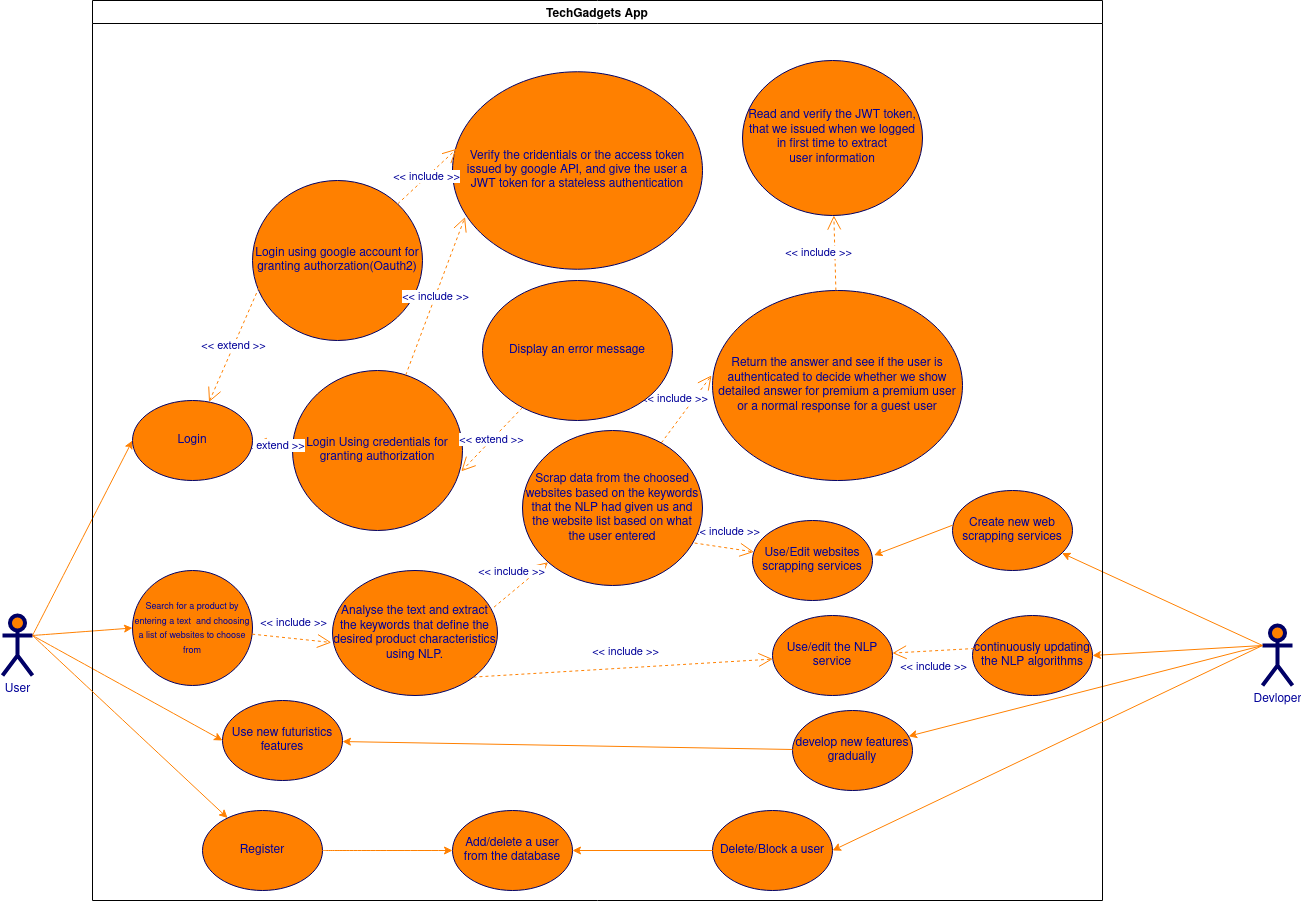
\includegraphics[scale=.4]{pics/Untitled Diagram(4).png}    
    \caption{Diagramme des cas d'utilisation}
    %\label{fig:my_label}
\end{figure}

\vfill


\section{Conception et analyse d'architecture générale de la solution: }

Après avoir présenté en quoi consiste l'application. Dans cette partie du chapitre, nous allons fournir l'architecture générale de notre application, y compris le workflow de l'interaction de l'utilisateur avec l'application, et comment le serveur gère la requête HTTP de l'utilisateur. Et les problèmes que l'architecture en microservice a résolus et vue generale sur le design pattern de nos microservices de l'application à l'aide de diagrammes pertinents car notre architecture est une architecture basée sur des microservices et chaque microservice est une petite application elle-même et on repete la meme design pattern pour chaque petite application.


\newpage




\subsection{différents éléments de l'architecture }

\textbf{Un microservice} : un microservice est une petite application qui représente une unité logique qui effectue une tâche logique dans l'ensemble de notre application, ces petites applications peuvent être hébergées sur différentes machines. lorsque nous avons besoin d'un microservice pour effectuer une opération, nous lui fournissons simplement l'entrée nécessaire et nous attendons la sortie. les flux d'entrée/sortie sont basés sur un protocole REST. Tous nos microservices seront basés sur une application Spring Boot ou une application Flask nous pouvons donc considérer nos microservices comme des ensembles des petites API. Mais ce qui en a fait des microservices, c'est le "Registry service" (Spring cloud registry serivce) qui fournit les informations nécessaires pour connecter ces microservices entre eux.

\begin{figure}[h]
\centering
    \centering
    \subfloat[\centering Microservice en Spring boot]{{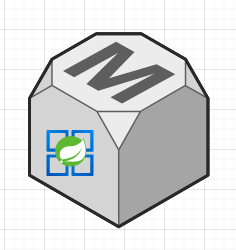
\includegraphics[width=.4\linewidth]{Selection_444.png}   }}%
    \qquad
    \subfloat[\centering Microserivce en Flask]{{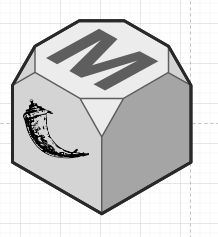
\includegraphics[width=.4\linewidth]{Selection_445.png}}}%
    \caption{Microservices}%
    \label{fig:example}%
\end{figure}



\textbf{ Opérateurs: }un opérateur est un ensemble des fonctions qui exécutent certaines tâches en Java ou en python sans avoir besoin d'appels externes pour d'autres microservices, pour le moment nous avons 3 types d'opérateurs l'opérateur NLP est un service qui analysera le texte de description que l'utilisateur émettra et le service "scrapping" qui extraira les données des sites Web ciblés ou le service de rechange qui utilisera des API externes pour extraire les données nécessaires dans le cas ou le service de "Scrapping" est hors-ligne ou il renvoie une erreur.



\begin{figure}[h]
\centering
    \centering
    \subfloat[\centering Opérateur qui fait des appels aux API'S externes ]{{
\includegraphics[scale=.5]{Selection_447.png}}}%
    \qquad
    \subfloat[\centering Opérateur qui fait fait du "Scrapping"]{{
\includegraphics[scale=.5]{Selection_448.png}}}%
    \caption{Opérateurs qui extraient les données nécessaires sur les produits }%
    \label{fig:example}%
\end{figure}

\textbf{Registry Service(Eureka)} : c'est un microservice qui offre des informations sur tous les autres microservices impliqués dans notre application. afin que nous puissions continuer à encadrer leurs activités, leur santé et leurs adresses dans le cloud. de cette façon si nous voulons les faire communiquer entre eux, nous pouvons simplement renvoyer leur nom sur le "Registry Service Eureka" et il nous fournira les informations nécessaires (adresse IP, port et instances disponibles, notez que chaque microservice peut avoir plusieurs instances) pour qu'on puisse appeler. Il est à que chaque microservice injecte ses informations sur le "Registry Service"

\begin{figure}[h]
\centering
    \centering
    \subfloat[\centering Eureka Discovery Service]{{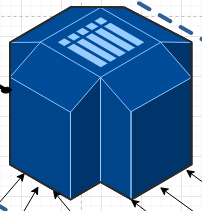
\includegraphics[width=.4\linewidth]{Selection_455.png}   }}%
    \qquad
\end{figure}


\textbf{Api gateway} : comme nous l'avons vu, chaque microservice peut être hébergé sur une machine différente donc une adresse IP différente. Le rôle de cette API Gateway est d'etre la passerelle c'est à dire; centraliser toutes les requêtes vers nos microservices. Au lieu d'appeler directement le microservice, nous utilisons une route de passerelle et nous mappons cette route au microservice à l'aide du Eureka. afin que le client envoie la requête à la même adresse IP et au même itinéraire même si le microservice souhaité change son adresse IP ou son port fréquemment, Eureka fournira toujours ces informations car le rôle d'eureka est de mapper le nom d'un mircoservice à son adresse meme s'il est hébergé sur le cloud et son adresse IP varie fréquemment, puis le "API GateWay" utilise ces donnes pour faire le routage. La centralisation des requêtes n'est pas la seule chose que fait la passerelle, nous pouvons aussi associer des règles à chaque route, telles que la journalisation des adresses IP des clients qui accèdent à une route spécifique ou sécuriser des routes et les rendons accessibles uniquement aux utilisateurs autorisés à y accéder. Nous centralisons donc la sécurité et la journalisation à un seul endroit afin qu'elles soient gérables ce qu'on appelle "Cross concern centralisation whit an Aspect oriented approach". 

\begin{figure}[h]
\centering
    \centering
    \subfloat[\centering API Gateway]{{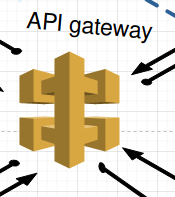
\includegraphics[width=.4\linewidth]{Selection_456.png}   }}%
    \qquad
\end{figure}

\textbf{Load balancer} : Comme nous l'avons vu, chaque microservice peut avoir plusieurs instances, donc le "load balancer" utilisera des algorithmes d'équilibrage pour répartir équitablement les requêtes entrantes sur les instances disponibles.

\begin{figure}[h]
\centering
    \centering
    \subfloat[\centering Load balancer]{{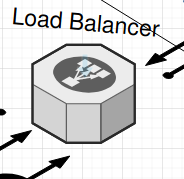
\includegraphics[width=.4\linewidth]{Selection_457.png}   }}%
    \qquad
\end{figure}

 
\textbf{Database} : la base de données est utilisée à des fins de stockage. Ici nous utilisons des bases de données MySql pour la production et des bases de données H2 pour les tests, il est à noter que la seule microservice qui utilise la base de donnes c'est le microservice d'authentification en utilisant hibernate pour faire la communication (ORM).
 
 \begin{figure}[h]
\centering
    \centering
    \subfloat[\centering Database]{{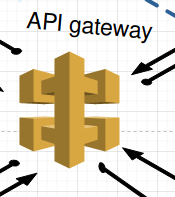
\includegraphics[width=.4\linewidth]{Selection_456.png}   }}%
    \qquad
\end{figure}

\textbf{Les relations entres les elements} :Il existe 3 types de relations entre notre composant :

-2 Flèche représentant un protocole REST pour la communication entre 2 composants.

-1 Flèche signifie injection de dépendance, nos opérateurs seront injectés dans les microservices.

-Flèche avec un symbole de verrouillage représente un itinéraire sécurisé afin que seuls les utilisateurs autorisés obtiendront la réponse 

 \begin{figure}[h]
\centering
    \centering
    \subfloat[\centering 2 Flèche]{{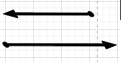
\includegraphics[width=.3\linewidth]{Selection_459.png}   }}%
    \qquad
     \centering
    \subfloat[\centering 1 Flèche]{{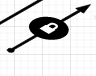
\includegraphics[width=.3\linewidth]{Selection_461.png}   }}%
    \qquad
     \centering
    \subfloat[\centering Flèche avec un symbole de verrouillage]{{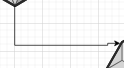
\includegraphics[width=.3\linewidth]{Selection_460.png}   }}%
\end{figure}

\section{Architecture générale et workflow: }

Maintenant que tous les éléments sont connus pour le lecteur, nous pouvons plonger dans l'architecture générale et voir comment chaque composant de notre application interagit avec d'autres composants. ainsi nous établirons les connaissances nécessaires pour voir pourquoi l'architecture des microservices est si puissante. et peut maintenant discuter quel type de problèmes elle résout pour notre cas d'utilisation, et aussi quel type de problème elle génère et comment nous allons gérer ces problèmes avec les technologies fournies par NETFLIX offert dans le framework Spring Cloud.


lien vers l'architecture: ( Voir fichier ci-joint, Architecture.html) 



\newpage
\hl{\textbf{Flux de travail idéal :}}

Le client envoie une requête HTTP comprenant le numéro de page, le texte de description ou les mots-clés du produit et ses informations d'identification (nom d'utilisateur et mot de passe ou jeton d'accès google) le microservice d'authentification validera les informations d'identification et émettra un jeton JWT au client contenant ses autorisations et ses informations personnelles à chaque fois qu'il envoie une requête au serveur il envoie cette jeton JWT, la passerelle verra si le jeton JWT est valide(Chiffrement et signature RSA). après cela, il déléguera la requête au microservice de l'utilisateur final qui déléguera le texte de description au microservice NLP pour extraire les mots-clés qui caractérisent le produit souhaité par le client, puis déléguera ces mots-clés au microservice qui récupère les données du produit à partir des sites Web externes comme amazon et ali-express, ce microservice vérifiera si le service de "Scrapping" fonctionne. si cela fonctionne, il récupérera les données en utilisant le "Scrapping", sinon il utilisera l'API externe (nous l'avons fait cette algorithme parce que l'API externe est un service payant). Ensuite, il enveloppera la réponse et la déléguera à l'utilisateur si l'utilisateur est authentifié, il lui fournira plus d'informations sur le produit(est ce que produit est "Best selling product", est-il en promotion, etc.), sinon il donnera un résultat normal.

Maintenant, avec le flux de l'application à l'esprit, nous allons parler des problèmes que l'architecture de microservices crée pour nous, et comment nous parvenons par la suite à résoudre ces problèmes.

\hl{\textbf{La sécurité par le modèle de session  :}}
En partant de l'idée que chaque microservice peut vivre dans une machine différente(Cloud), la solution typique de "session" pour l'autorisation et le suivi des utilisateurs authentifiés n'est plus valide et nous devons rechercher une solution "Statless", c'est-à-dire ne pas conserver les informations des utilisateurs en mémoire, mais plutot les conserver chez une autre service ou l'utilisateur lui meme. pour résoudre ce problème, nous avons utilisé le jeton JWT et les protocoles Oauth2 (on a utilise, ce du google).


\hl{\textbf{Orchestration des microserivces :}}
Chaque microservice est une application autonome, pour garder une trace de toutes ces applications, nous avons utilisé la solution que Netflix a développé "Spring cloud". qui fournissent la "Spring cloud API Gateway" pour centraliser les requetes et le serveur de découverte Eureka en tant "Service Registry", et "Health Actuator" pour pour tracer l'état de santé des microservices.

\hl{\textbf{Microservices applications and Boostraping :}}
chaque microservice est une petite application donc a chque fois on veut creer un microservice il faut bcp des configuration, on a resourdre ca en utilisant spring boot et flask parcque ces deux framework minimiser la configuration necessaire pour demarer une application. meme ils generent les dependences qu'on aura besoin.

\hl{\textbf{Error Handling and circuits Breaker:}}
Imaginez si un microservice génère une erreur, cette erreur sera transmise au microservice appelant en tant que réponse HTTP avec le statut 500 en tant qu'erreur interne, et comme cela, nous ne pouvons pas savoir où nous obtenons cette erreur ou quelle est la cause de l'erreur, pour résoudre ce problème nous avons utilisé "Spring Cloud cricuit breaker" basé sur la "résillance", il coupera le circuit et donnera une réponse directement au client en cassant le modèle d'appelant appelé.



\hl{\textbf{Pourqoui on a utliser les microservices:}}


\hl{\textbf{Résilience:}}
Les microservices nous fournissent un grand nombre de fonctionnalités, l'une est la résilience si nous voulons ajouter une nouvelle fonctionnalité ou déboguer un problème, nous n'avons pas besoin de déconnecter notre application mais uniquement le service concerné, et comme vous savez notre application dependent largement des services externes.

\hl{\textbf{"Cloud native architecture":}}
"Cloud native application, or Distrbuted System native application" nous aide à augmenter notre base d'utilisateurs, de sorte que notre application sera en mesure de prendre en charge une énorme base d'utilisateurs, et même pour le "scraping", il faut qu'on utilise plusieurs IP adresse pour éviter le blocquage.

\hl{\textbf{"Ready production features: "}}
Concentrez-vous sur la production, chaque membre de l'équipe utilisera les technologies qu'il aime utiliser.
Composants réutilisables, chaque microservice sera dédié à une seule tâche logique afin que nous puissions le réutiliser dans d'autres projets.



\section{Design patterns: }
dans cette section, nous parlerons des modèles de conception que nous avons utilisés pour développer nos micros services, on va étudier une seule micro service(Celui d'authentification) et les autres doivent suivi le même design patter


\subsection{Inversion of control and dependecny injection:}
Le framework spring est base sur ces deux concepts qui offrent une "Designe pattern" pret pour la production

\subsection{MVC modele:}
Nous avons utilisé le célèbre modèle MVC(avec des petites customisation parce qu'on a pas du "VIEW" ici)avec une gestion d'erreur personnalisée pour intégrer « Cicuit Breaker » 

\begin{figure}[h]
\centering
    \centering
    \subfloat[\centering MVC:application]{{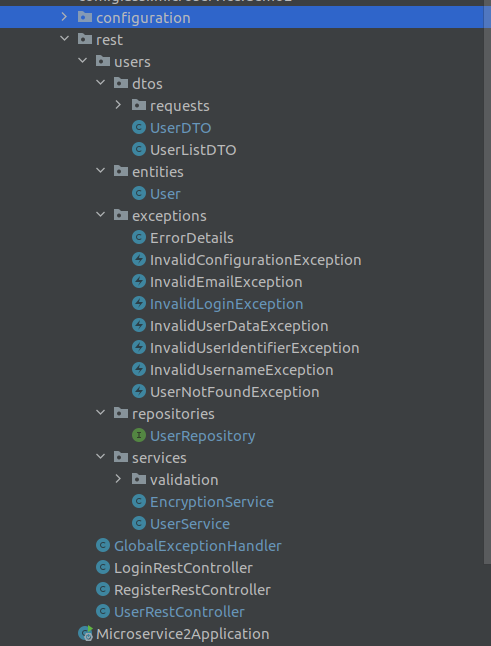
\includegraphics[width=.3\linewidth]{Selection_462.png}   }}%
\end{figure}

\hl{\textbf{"DTOS package classes":}}
Des classes qui sont dédiées à la serialisation des objets JSON que le client envoie à des objets "POJO"


\hl{\textbf{"ENTITES and REPOSITORIES package classes":}}
On peut donc utiliser n'importe quelle base de données, car c'est Hibernate qui crée les requêtes sql en transmettant votre code java basé sur la spécification JPA. 

\hl{\textbf{"exceptions package classes":}}
Des classes qui sont dediees a la manipulation des errours et déclenchement du "Circuit Breaker".

\hl{\textbf{"SERVICES package classes and Controller":}}
Ces classes représentent le contrôleur qu'il délègue la requête aux routes propres et les services sont ceux qui contiennent notre couche métie.


\subsection{ORM}
Un mapping objet-relationnel (en anglais object-relational mapping ou ORM) est un type de programme informatique qui se place en interface entre un programme applicatif et une base de données relationnelle pour simuler une base de données orientée objet. Ce programme définit des correspondances entre les schémas de la base de données et les classes du programme applicatif. On pourrait le désigner par là, « comme une couche d'abstraction entre le monde objet et monde relationnel ». Du fait de sa fonction, on retrouve ce type de programme dans un grand nombre de frameworks sous la forme de composant ORM qui a été soit développé, soit intégré depuis une solution externe. 

\\
\begin{figure}[!htb] 
\begin{center} 
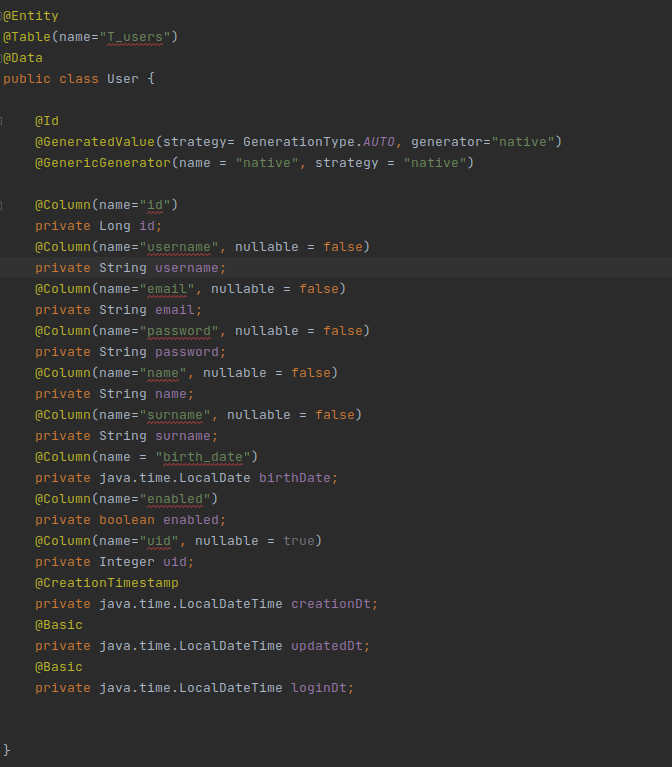
\includegraphics[scale=.5]{Selection_463.png}    
\end{center} 
\caption{ORM Entity of Authentication Microservice} 
\end{figure}  \FloatBarrier
\\

\subsection{Unit testing: Test driven devloppment}
Pour uni testing on a utilisé JUNIT et Mockito, la seule micro service qui a ces unis test totalement faites est celui de l'authentification, lors de l'ecriture de ce microservice on a suivi "Test Driven Devloppement Approach" 

\\
\begin{figure}[!htb] 
\begin{center} 
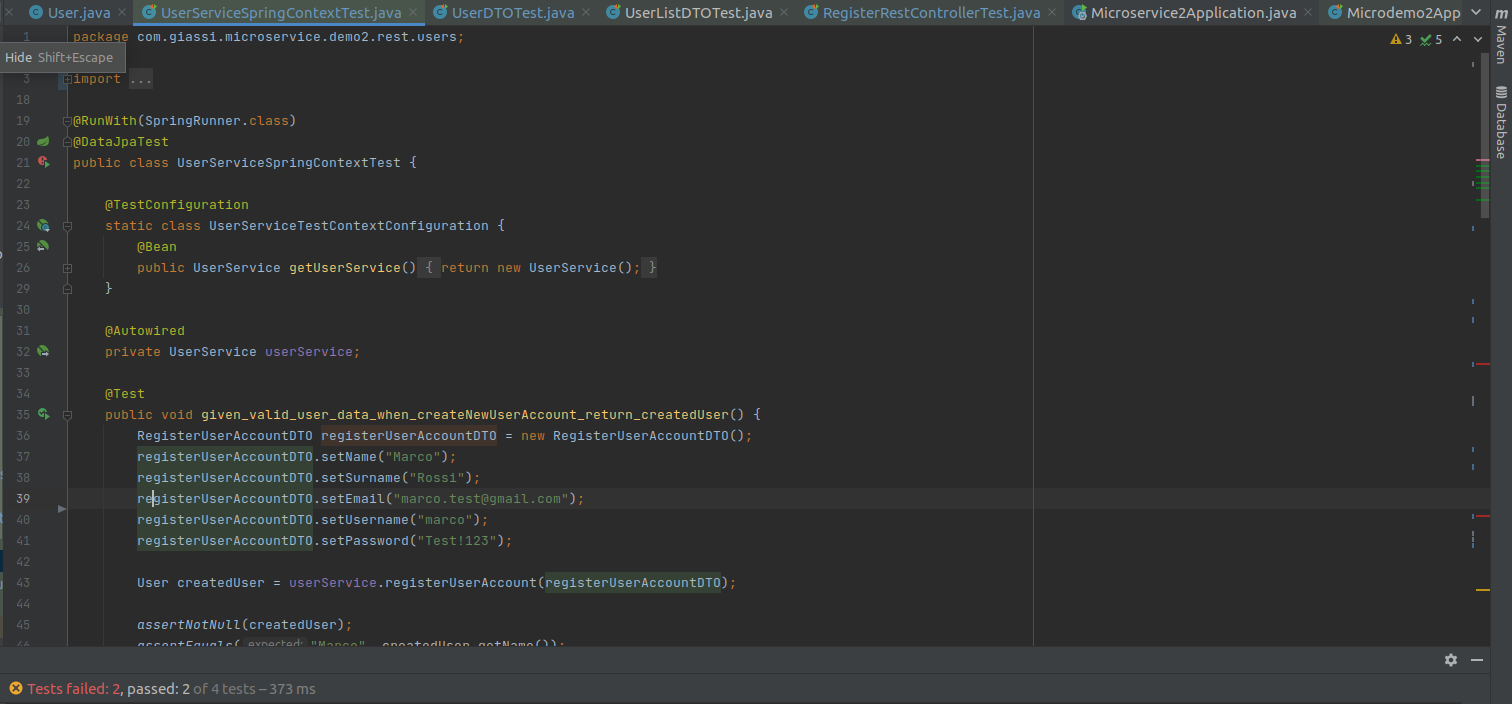
\includegraphics[scale=.6]{Selection_470.png}    
\end{center} 
\caption{Test unitaires}
\end{figure}  \FloatBarrier
\\
\section{Machine Learning}

Notre platfrome doit être capable de recommander les appareils électroniques d'après une description d'utilisateur. Bien entendu le "Natural Langage Processing" sera la technologie qu'on utilise pour résoudre cette problématique, cependant on doit passer par plusieurs étapes pour réaliser un modèle capable de réaliser cette tâche.

\subsection{Préparation des données }

\textbf Pour ce projet, l’ensemble de données électroniques se compose de commentaires et d’informations sur les produits d’amazon
Cet ensemble de données comprend des évaluations (cotes, texte, votes sur l’utilité) et des produits.
les métadonnées (descriptions, renseignements sur la catégorie, prix, marque et caractéristiques de l’image)..


\begin{figure}[!htb] 
\begin{center} 
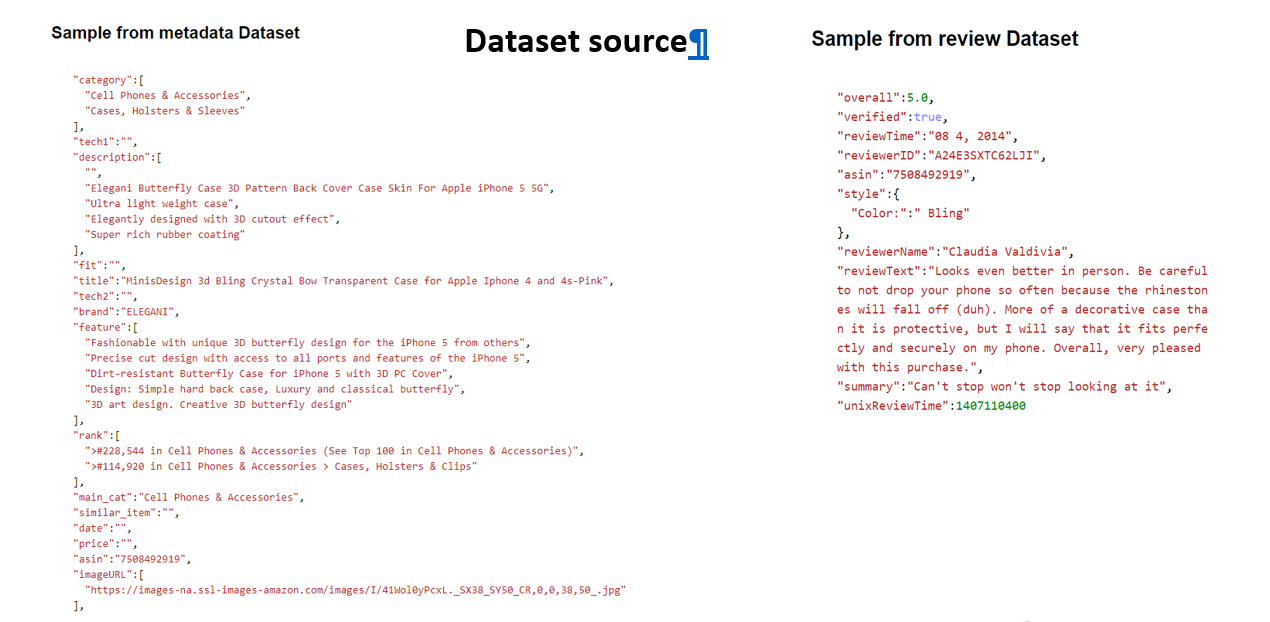
\includegraphics[scale=0.55]{pics/screens/6.png}
\end{center} 
\caption{Dataset Sample} 
\end{figure}  \FloatBarrier
\\
\\
\begin{figure}[!htb] 
\begin{center} 
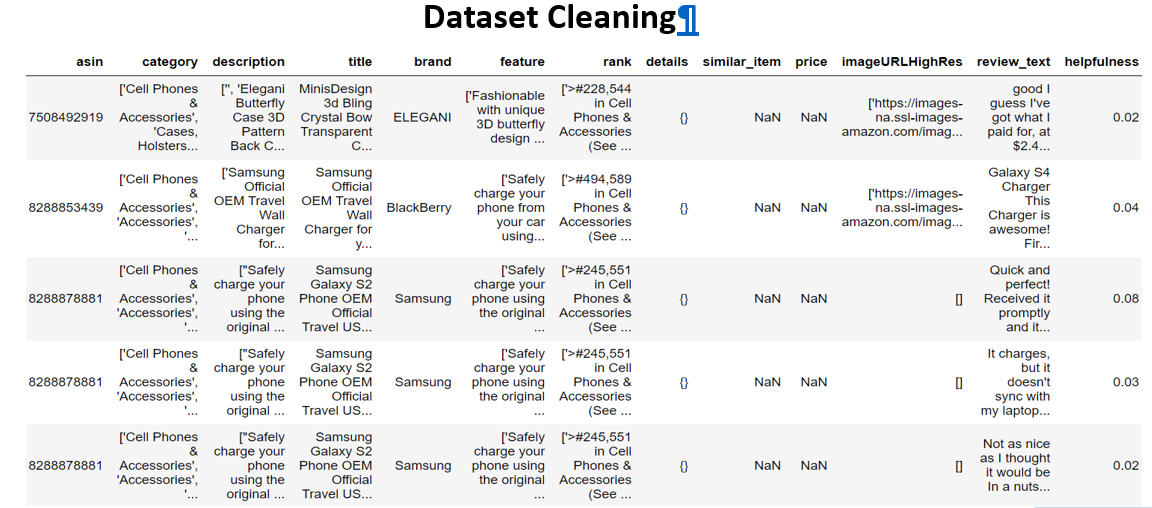
\includegraphics[scale=.6]{pics/screens/7.png}
\end{center} 
\caption{Cleaned Dataset} 
\end{figure}  \FloatBarrier
\\
\subsection{Prétraitement de texte  }

\textbf Puisque le texte est la forme la plus peu structurée de toutes les données disponibles, divers types de bruit sont
présent dans celui-ci et les données ne sont pas facilement analysables sans aucun prétraitement. L’ensemble du processus
de nettoyage et de normalisation du texte, le rendant sans bruit et prêt pour l’analyse est connu comme
prétraitement du texte. Dans cette section, le prétraitement du texte suivant a été appliqué.

\\
\begin{figure}[!htb] 
\begin{center} 
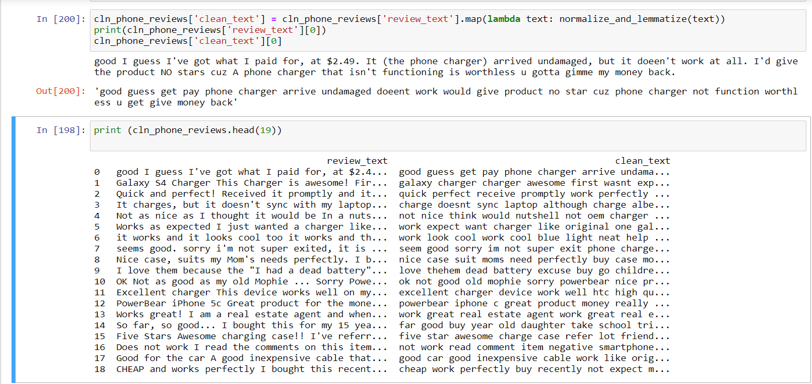
\includegraphics[scale=0.8]{pics/screens/8.png}
\end{center} 
\caption{Example of Normalization} 
\end{figure}  \FloatBarrier
\\
\\
\begin{figure}[!htb] 
\begin{center} 
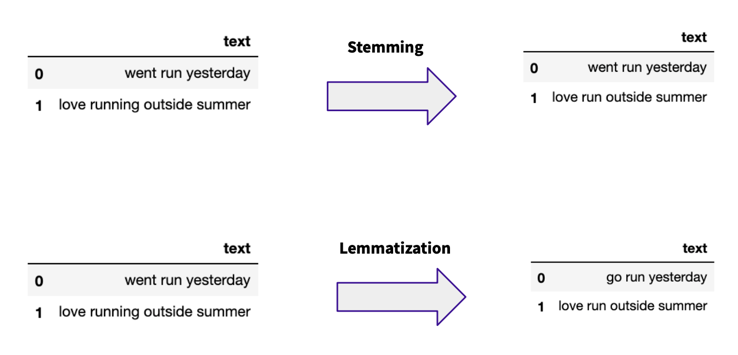
\includegraphics[scale=0.9]{pics/screens/9.png}
\end{center} 
\caption{Stemming vs Lemmatizationt} 
\end{figure}  \FloatBarrier
\\
\subsection{Features Extraction & Sentiment Analysis }

\textbf Les modèles d’apprentissage automatique prennent des valeurs numériques comme entrée. Les révisions sont faites de phrases,
donc afin d’extraire des modèles à partir des données; nous devons trouver un moyen de les représenter d’une manière que
l’algorithme d’apprentissage automatique peut comprendre, i.e. comme une liste de nombres. \\

\\
\begin{figure}[!htb] 
\begin{center} 
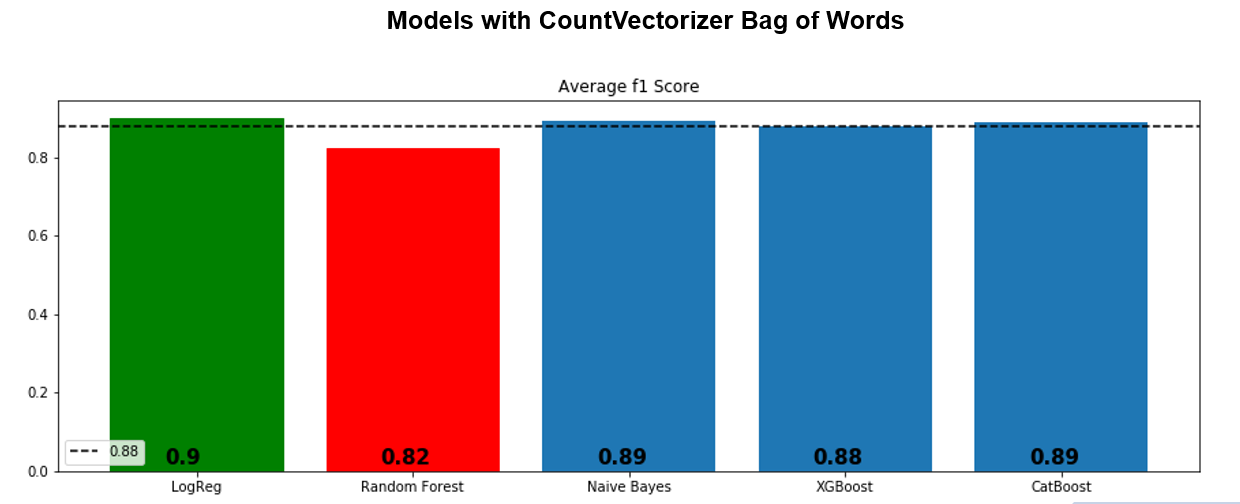
\includegraphics[scale=0.5]{pics/screens/11.png}
\end{center} 
\caption{Models Testing} 
\end{figure}  \FloatBarrier
\\


Feature engineering consiste à utiliser la connaissance du domaine des données pour créer des fonctions qui :
rendre les algorithmes d’apprentissage automatique fonctionnable. Les "Features" sont généralement de nature numérique et peuvent être valeurs numériques absolues ou caractéristiques catégoriques qui peuvent être encodées en tant que caractéristiques binaires pour chaque dans la liste à l’aide d’un processus appelé encodage one-hot. Le processus d’extraction et la sélection des caractéristiques est à la fois l’art et la science, et ce processus s’appelle l’extraction de caractéristiques ou de caractéristiques ingénierie.\\

\\

\\
\begin{figure}[!htb] 
\begin{center} 
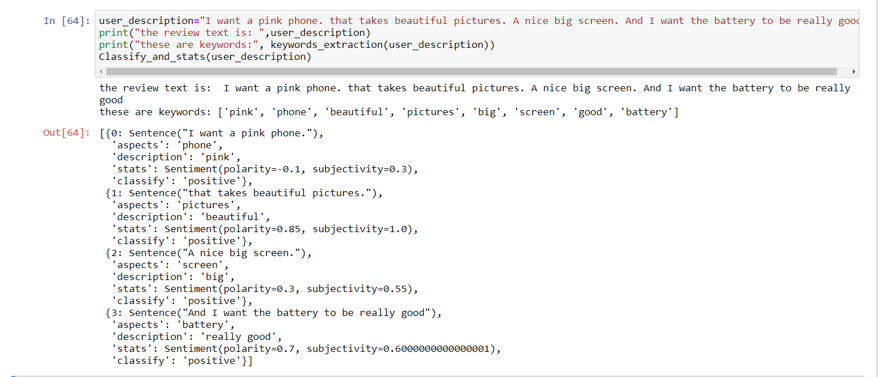
\includegraphics[width=1\linewidth]{pics/screens/10.png}
\end{center} 
\caption{Aspect Based Sentiment Analysis} 
\end{figure}  \FloatBarrier
\\
Dans le cadre de ce projet, Bag of Words model, TF-IDF, Hashing Vectorizer, Word2Vec et ajout des mots les plus courants dans la liste des mots clés, SMOTE, PCA et SVD tronqué techniques en modèles de classification dans les sections suivantes dans le cadre de l’ingénierie des caractéristiques et la sélection. \\


 \\*


\section{Conclusion}

Dans ce chapitre nous avons présenté de manière globale les principales étapes de l'analyse et la conception de notre application suivant les différentes schémas, afin de concilier la phase de mise en œuvre. Le prochains chapitre sera consacré à la phase de développement de notre application.

\begin{center}
\chapter{Mise en oeuvre}    
\end{center}


Après avoir réalisé une conception répondant au mieux aux besoins de notre application, nous commençons la partie implémentation de l'application que nous avons développée, en exposant les différents outils de développement et langages utilisés lors de la production de nos application ainsi que les résultats obtenu.\\


\section{outils utilisés :}
\centuring
\subsection{HTML et CSS :}
\begin{center}
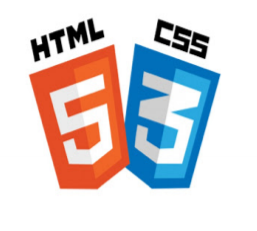
\includegraphics[scale=1]{pics/html+css.png}    
\end{center}


HTML, HyperText Markup Language, donne une structure et un sens au contenu en définissant ce contenu par principe de balisage comme, par exemple, des titres, des paragraphes ou des images.. etc . \\
 CSS, ou Feuilles de style en cascade, est un langage de présentation créé pour styliser l'apparence du contenu, en utilisant, par exemple, des polices ou des couleurs. \\

\subsection{Bootstrap 5:}
\\
\begin{center}
\includegraphics[scale=.2]{pics/bootstrap.png}    
\end{center}


Bootstrap est un Front-End Framework développé par l'équipe du réseau social Twitter. Proposé en open source (sous licence MIT), ce Framework utilisant les langages HTML, CSS et JavaScript fournit aux développeurs des outils pour créer un site facilement. \\

Il est pensé pour développer des sites avec un design responsive, qui s'adapte à tout type d'écran, et en priorité pour les smartphones. Il fournit des outils avec des styles déjà en place pour des typographies, des boutons, des interfaces de navigation et bien d'autres encore.  \\

\subsection{Angular :}
\begin{center}

\includegraphics[scale=0.5]{pics/Angular.png}    
\end{center}
Angular s’inscrit définitivement dans une approche moderne de la création d’applications web « One page » et d’interfaces utilisateurs. Orienté objet, ce Framework MVC exploite le langage Typescript (langage compilé qui va générer du Javascript). Avec Angular, la logique applicative est insérée directement dans le HTML par l’intermédiaire d’éléments ou d’attributs (principe du data-binding).\\

            => TypeScript:\\
TypeScript est un langage open-source pris en charge par Microsoft, qui s’appuie sur JavaScript en ajoutant une fonction de type statique facultative. Les types fournissent un moyen de structurer et de valider son code avant de l’exécuter. \\

            => gapi ( google API) pour une authentification oauth2) \\
Le contrôle d'accès pour les API Google Cloud comprend l'authentification, l'autorisation et l'audit. L'authentification établit qui vous êtes, l'autorisation détermine ce que vous pouvez faire et les audits enregistrent ce que vous avez fait. \\


\subsection{Spring Cloud :}

\begin{center}

\includegraphics[scale=1]{pics/Spring-Cloud.png}    
\end{center}
Spring Boot est un framework de développement JAVA. C'est une déclinaison du framework classique de Spring qui permet essentiellement de réaliser des micro services (ce sont la majeure partie du temps des services web qui sont regroupés en API). \\

            => Spring cloud circuit breaker(Resilience4J) \\
Spring Cloud Circuit breaker provides an abstraction across different circuit breaker implementations. It provides a consistent API to use in your applications allowing you the developer to choose the circuit breaker implementation that best fits your needs for your app. \\ 

            => Eureka discovery service \\
C'est un service développé en Java par Netflix, dont le rôle est de gérer l'enregistrement et la localisation de services à des fins de load balancing et de failover. Sa très bonne intégration avec Spring Boot fait de lui un très bon choix de Service Registry dans le monde des micro-services Java. \\

\subsection{Python :}
\begin{center}

\includegraphics[scale=1]{pics/Python.png}    
\end{center}

Python est particulièrement populaire pour l'analyse de données et la Machine Learning, mais aussi pour le développement web backend. Ce langage est aussi utilisé pour scraper des donnes du web et développer des outils de productivité. \\
         
         =>json \\
Python est livré avec un paquet intégré appelé json pour encoder et décoder les données JSON. Le processus d'encodage de JSON est généralement appelé sérialisation. Ce terme désigne la transformation de données en une série d'octets (donc en série) à stocker ou à transmettre sur un réseau. \\
         

\subsection{Pandas :}
\begin{center}

\includegraphics[scale=1]{pics/Pandas.png}    
\end{center}


Pandas est une bibliothèque écrite pour le langage de programmation Python permettant la manipulation et l'analyse des données. Elle propose en particulier des structures de données et des opérations de manipulation de tableaux numériques et de séries temporelles. \\

\subsection{NLTK :}
\begin{center}

\includegraphics[scale=1.3]{pics/NLTK.png}    
\end{center}

NLTK est une plate-forme pour manipuler les données du langage humain. NLTK guide le lecteur à travers les principes fondamentaux de l’écriture de programmes Python, le travail avec les corpus, la catégorisation du texte, l’analyse de la structure linguistique, et plus encore..\\

\pagebreak
\section{Réalisation : }
\\
Pour bien comprendre toutes les fonctionalités de l'application on suit deux scénarios selon les acteurs: \\
\subsection{Guest :}
à l'ouverture de l'application le patient voit  la page d'acceuil suivante  où il peut faire sa recherche, Pour faire sa recherche , le Guest peut écrire juste une description generale du produit et (Figure 3.2 ) :\\

\begin{figure}[h]
    \centering
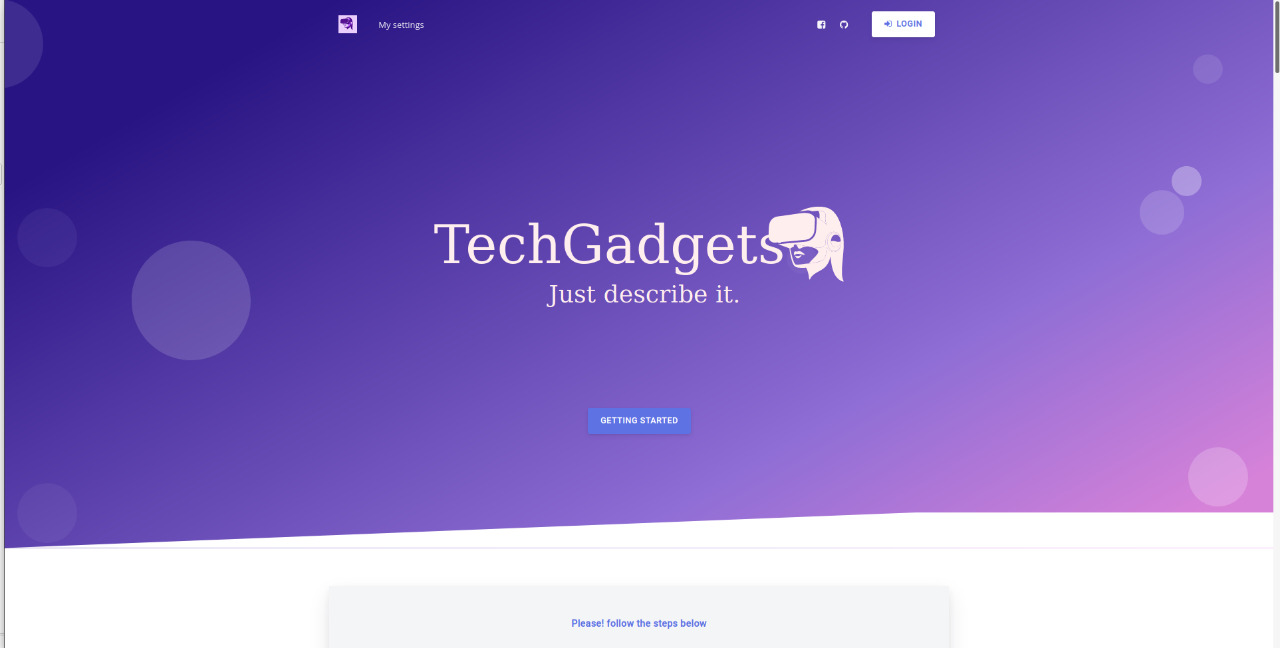
\includegraphics[scale=.4]{pics/screens/1.png}
\caption{Page d'accueil/ propriétés TechGadgets}
\\


\end{figure}
\vfill
\begin{figure}[h]
    \centering
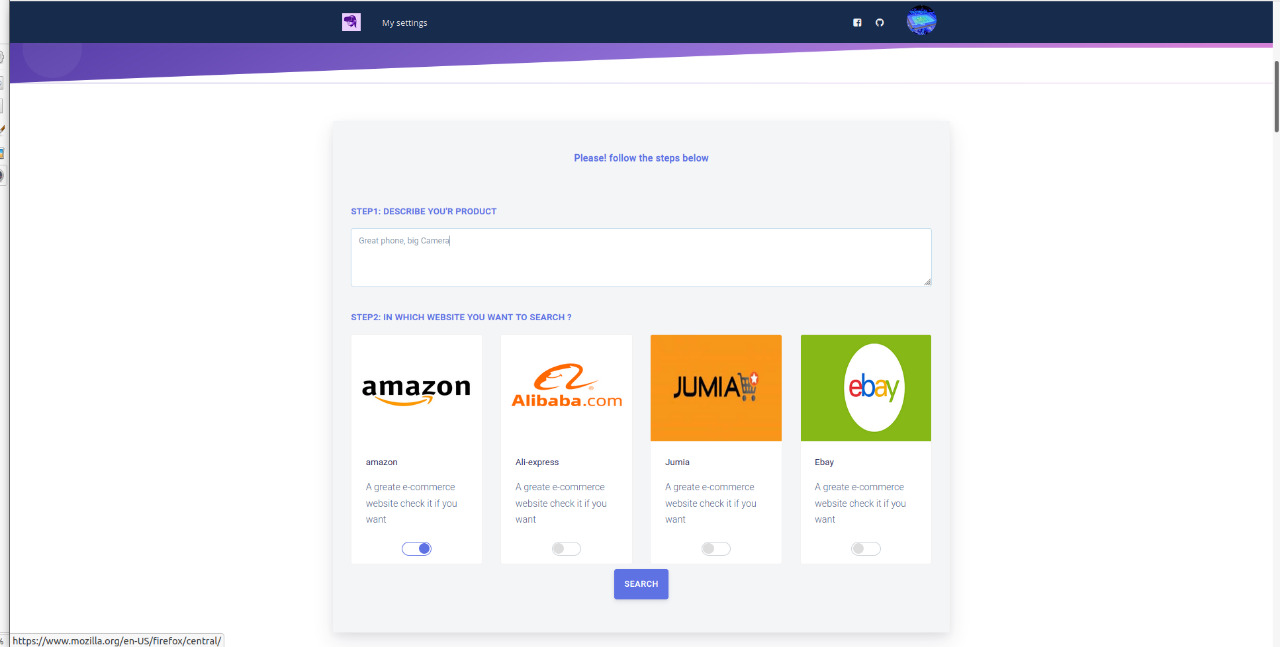
\includegraphics[scale=.4]{pics/screens/2.png}
\caption{Page d'accueil/ barre recherche}
\end{figure}
\begin{figure}[!T]
   \centering
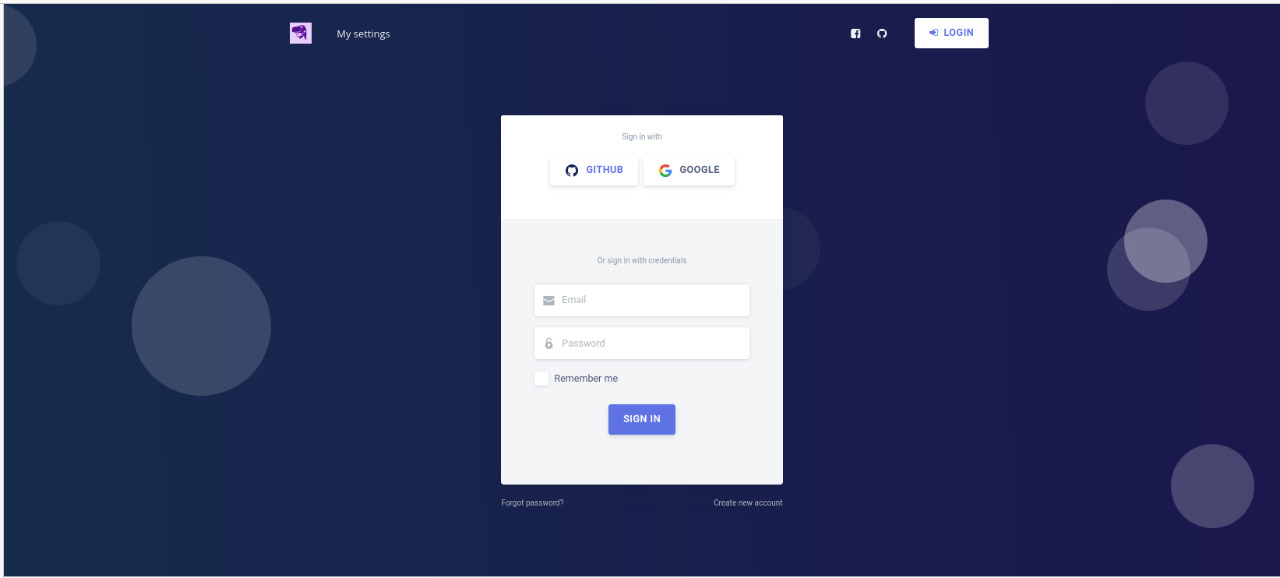
\includegraphics[scale=.4]{pics/screens/4.png}
\caption{Page d'accueil/ Login et Signup}
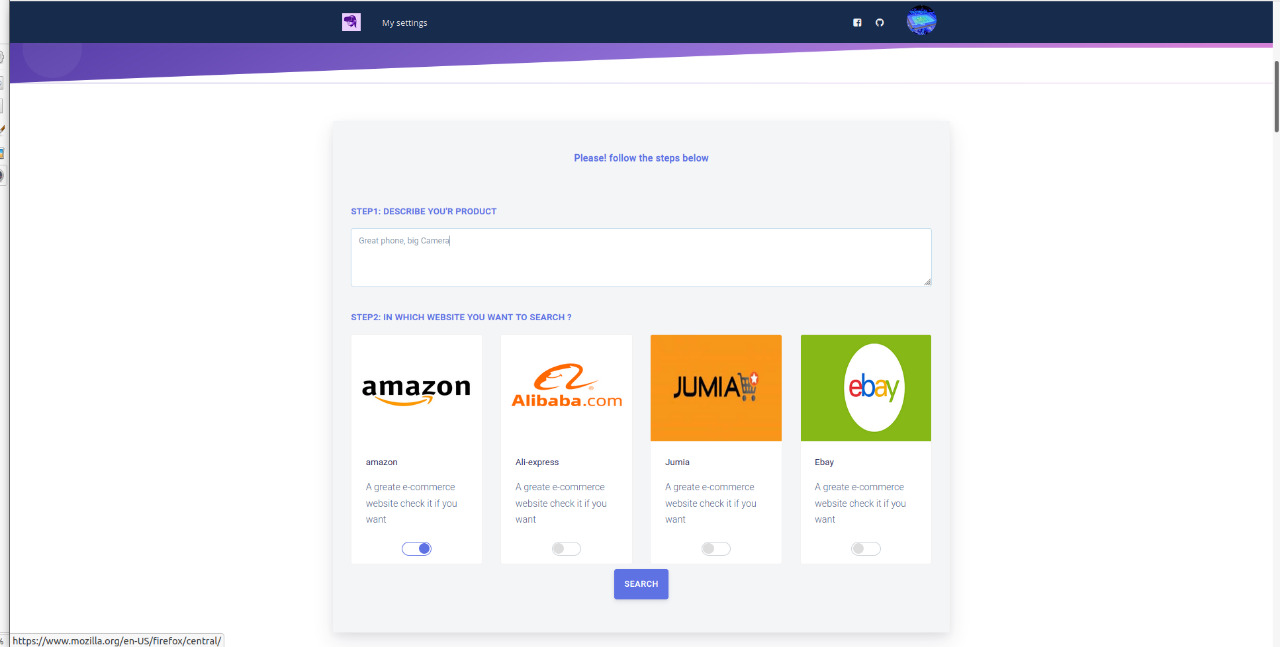
\includegraphics[scale=.4]{pics/screens/2.png}
\caption{Page d'accueil/ barre recherche}
\end{figure}
\pagebreak
\begin{figure}[!T]
   \centering
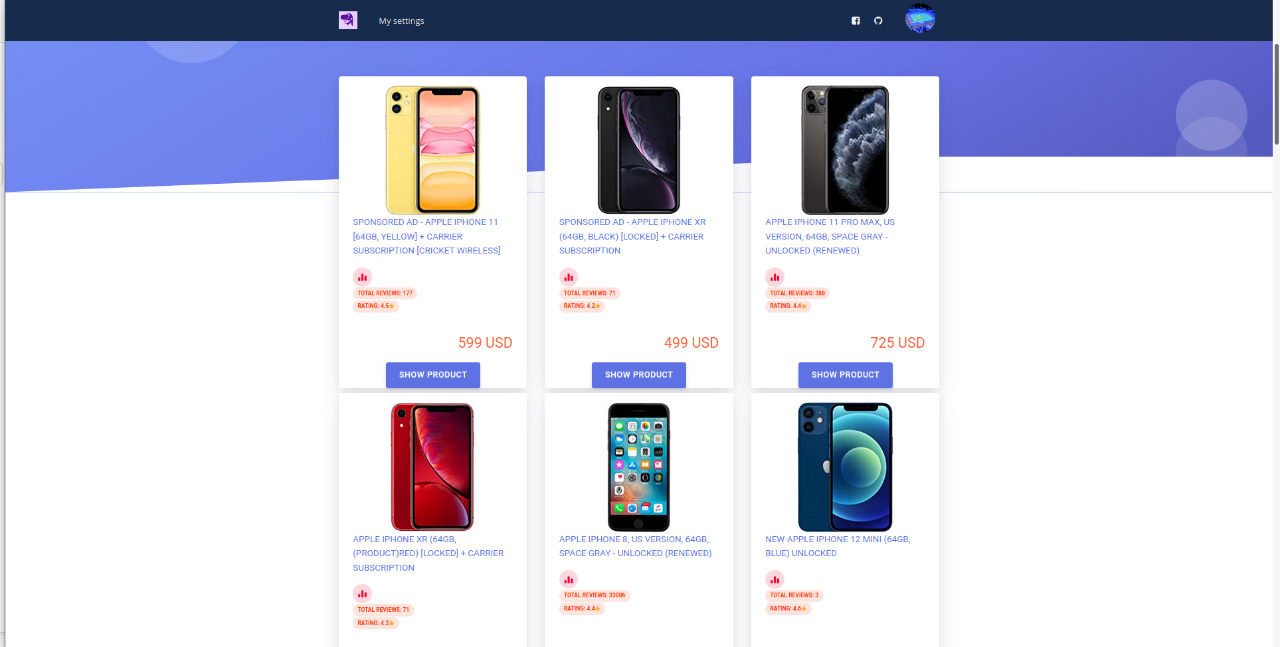
\includegraphics[scale=.4]{pics/screens/3.png}
    \caption{Les produits recommandés}  
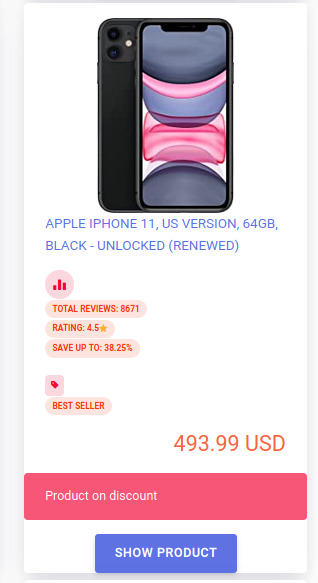
\includegraphics[scale=.4]{pics/screens/5.png}
    \caption{Les détails specifics aux abonnées}  
\end{figure}




\\


\newpage

\begin{center}
    \chapter*{Conclusion générale}
\end{center}
\addcontentsline{toc}{chapter}{Conclusion générale}
Le travail que nous avons fait a consisté sur la réalisation d'une application web de recommandation . Nous avons fait une petite analyse aux situations des utilisateur. nous avons fournit aussi l'architecture générale de notre application, y compris le workflow de l'interaction de l'utilisateur avec l'application et le les details de notre model de Machine Learning. \\

Ce projet nous a permis d'acquérir une expérience personnelle et professionnelle. Il nous a été bénéfique  car nous avons eu la chance d'améliorer nos connaissances en développement web, Architecture Microservices, Machine Learning et aussi de développer une capacité de résolution des problèmes vu qu'on a eu une difficulté dans le choix du framework le plus convenable pour notre application ainsi dans la recherche des solutions des erreurs qui , évidement, apparaissent partout dans le code.\\

Arrivant à ce point là, nous restons encore ambitieux pour faire des améliorations qu’on n’a pas eu le temps pour les réaliser dans la période du module à savoir : \\

\begin{itemize}
    \item L'authentification d'utilisateur par Amazon Acoount
    \item L'integration des platfrome des avis techniques 
    \item la possibilité aux utilisateurs de contribuer à notre Model
\end{itemize}
